\section{Modeling \pp collisions}
Theoretical predictions of \pp collisions are an important tool for understanding physical processes and modeling observables studied at the LHC. These predictions are based on an underlying proton model and calculations are performed from approximations at different energy scales. Precision measurements such as the one in this thesis provide important information to further refine these models and calculations. This chapter describes the general methods for modeling proton-proton collisions as well as details about \W and \Z boson production at the LHC.
\subsection{Simulating \pp interactions}
In collisions at very low energies, protons can be approximated as electrically charged objects. At higher energies, such as those at the LHC, the structure within protons begins to have an important role for the scattering process. \W and \Z bosons are produced from the interaction of quarks and gluons (both also referred to as partons) within the proton\cite{PhysRevLett.23.930,PhysRevLett.23.935}. The contributions of the partons to the proton's structure are described by parton distribution functions (PDFs). The PDFs, $f_i(x,Q^2)$, give the probability of finding a parton of carrying a fraction $x$ of the proton momentum. The PDFs cannot be calculated directly, and are instead determined from experimental data. Valence quarks, sea quarks, and gluons within the proton are described by the PDFs. 

For hard scattering processes such as \W and \Z boson production, the momentum transfer, $Q$ is high. Due to the asymptotic freedom of QCD, the coupling constant $\alpha_S(Q^2)$ is small, and perturbative calculations are effective. The highest order calculation currently available for the \W and \Z production is next-to-next-to-leading order (NNLO)\cite{Anastasiou:2003ds}. 

In the perturbative expansions, initial-state radiation of soft and collinear gluons produces logarithmic terms which cause singularities and divergences in the calculations. To accommodate this effect, the calculation can be split into perturbative and non-perturbative regimes. The factorization theorem ensures that the hard process is independent of the intial-state radiation, and separates the QCD calculations at a factorization scale, $\mu_F$. This allows the singularities due to the soft gluon emissions to be factored out and contained within the PDFs~\cite{Collins:1989gx}. The PDF dependence on the factorization scale is determined by the Dokshitzer–Gribov– Lipatov–Altarelli–Parisi (DGLAP) equations. The DGLAP equations introduce a $\mu_F$ dependence to the scale-independent PDFs by including initial-state soft radiation, and provide an evolution of the PDFs over different factorization scales\cite{Gribov:1972ri,Dokshitzer:1977sg}.  Equation~\ref{eq:factorization_xsec} shows the factorized cross section calculation. The first section includes the PDFs, $f_{a}$ and $f_{b}$, evaluated at the factorization scale $\mu_F$, for partons $a$ and $b$, each carrying fractions $x_a$ and $x_b$ of the proton momentum. The second half describes the hard scattering between the two partons, where the cross section, $\hat{\sigma}$, is expanded perturbatively.  
\begin{equation}
\begin{aligned}
\sigma_{p_a p_b \rightarrow n} &= \sum_{a,b}{\int{dx_a dx_b f_{a}(x_a, \mu^2_F)f_{b}(x_b, \mu^2_F)}} \\ &\times[\hat{\sigma}_{LO}(x_a x_b s, \mu^2_R, \mu^2_F)+\alpha_S \hat{\sigma}_{NLO}(x_a x_b s, \mu^2_R, \mu^2_F) + \cdots]
    \label{eq:factorization_xsec}
\end{aligned}
\end{equation}
Parton-parton cross sections ($\hat{\sigma}$) are determined by numerically integrating matrix element calculations by using a Monte Carlo (MC) process to sample the phase space.

Matrix element calculation breaks down for soft and collinear final states. Instead, parton shower models are used to produce the final-states at non-perturbative scales. Showering is modeled as series of radiative steps, with partons branching into consecutively lower energy state: $q\rightarrow gq$, $g\rightarrow gg$, and $g\rightarrow q\bar{q}$ for QCD. Branching probability at a scale $Q^2$ is determined by evolving the splitting functions using the DGLAP equations. Additionally, QED interactions ($q\rightarrow q\gamma$ and $l\rightarrow l\gamma$) are included in the shower modeling. Parton showering continues to the scale $\Lambda\sim 200~\mathrm{MeV}$, where bare partons are hadronized into color-neutral hadrons. Then the unstable hadrons are decayed according to branching ratios. Factorization and a hard scatter process, along with subsequent parton showering and hadronization is illustrated in Figure~\ref{fig:sm:evtgen}.

% Multiple collaborations exist to provide tools capable of performing the different calculations described above. 

\begin{figure}
\centering
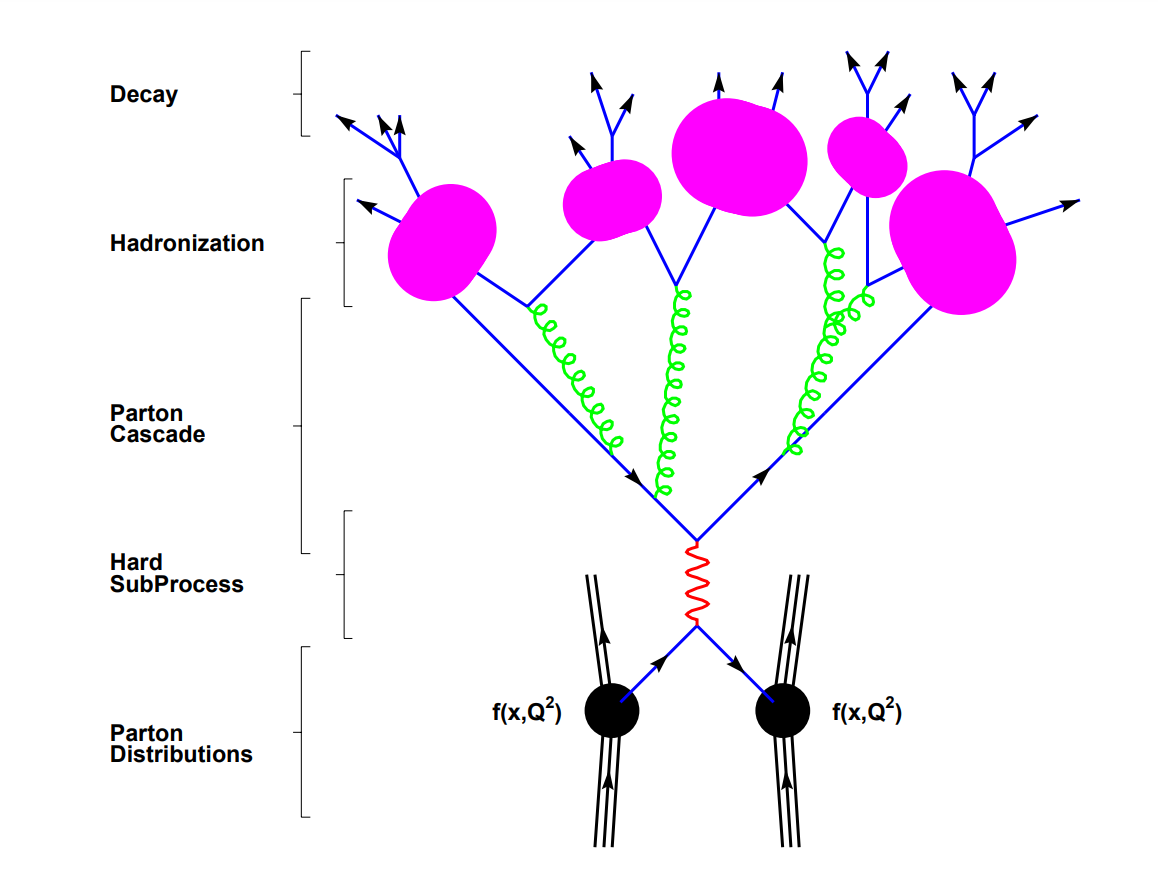
\includegraphics[width=0.6\linewidth]{plots/SM/evtgenerator.PNG}
%   \caption{1a}
%   \label{fig:Eff:el:5TeV:GSFSel:pos
\caption{Illustration of a hard-scatter process. \protect\cite{Dobbs:2001ck}}
\label{fig:sm:evtgen}
\end{figure}
% %%%%%%%%%%%%%%%% vvvvvvv finish later
% %% Comment back in later 
\subsection{\W and \Z production at the LHC}
In the \pp collisions, the bosons are produced through the interaction of quarks and gluons within the protons \cite{}. The primary production modes for the \W and \Z bosons is through the Drell-Yann process, predonminantly $u\bar{u}, d\bar{d}\rightarrow Z$,  $u\bar{d}\rightarrow W^+$,  and $d\bar{u}\rightarrow W^-$. 

Figure~\ref{fig:sm:summary:xVsQ2}.





% %%%% figure
\begin{figure}
\centering
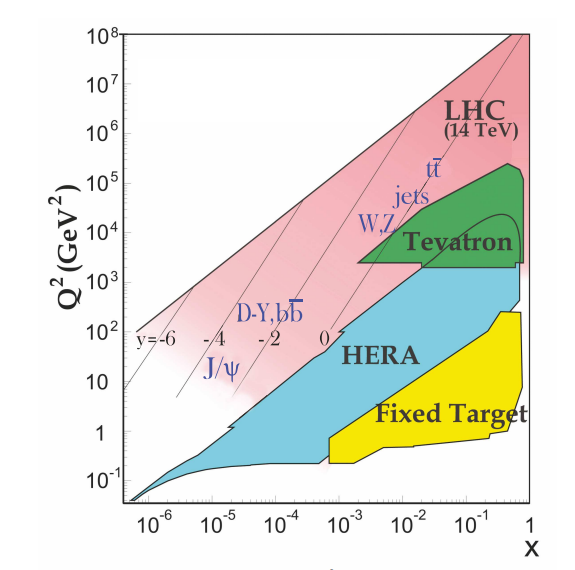
\includegraphics[width=0.6\linewidth]{plots/SM/structure_probes.PNG}
%   \caption{1a}
%   \label{fig:Eff:el:5TeV:GSFSel:pos
\caption{Phase space of Bjorken-x and $Q^2$ available at the LHC and other experiments. \pp collisions at the LHC can probe very high $Q^2$. \protect\cite{PhysRevD.98.030001}}
\label{fig:sm:summary:xVsQ2}
\end{figure}

Measurements of \W and \Z boson production at the LHC provide information related to different PDFs due to the different relative contribution of each flavor in the production.

Contributions of different quark flavors to \W and \Z production over a range of rapidities is shown in Figure~\ref{fig:wz_rapidity}. 

\begin{figure}[htbp]
\centering
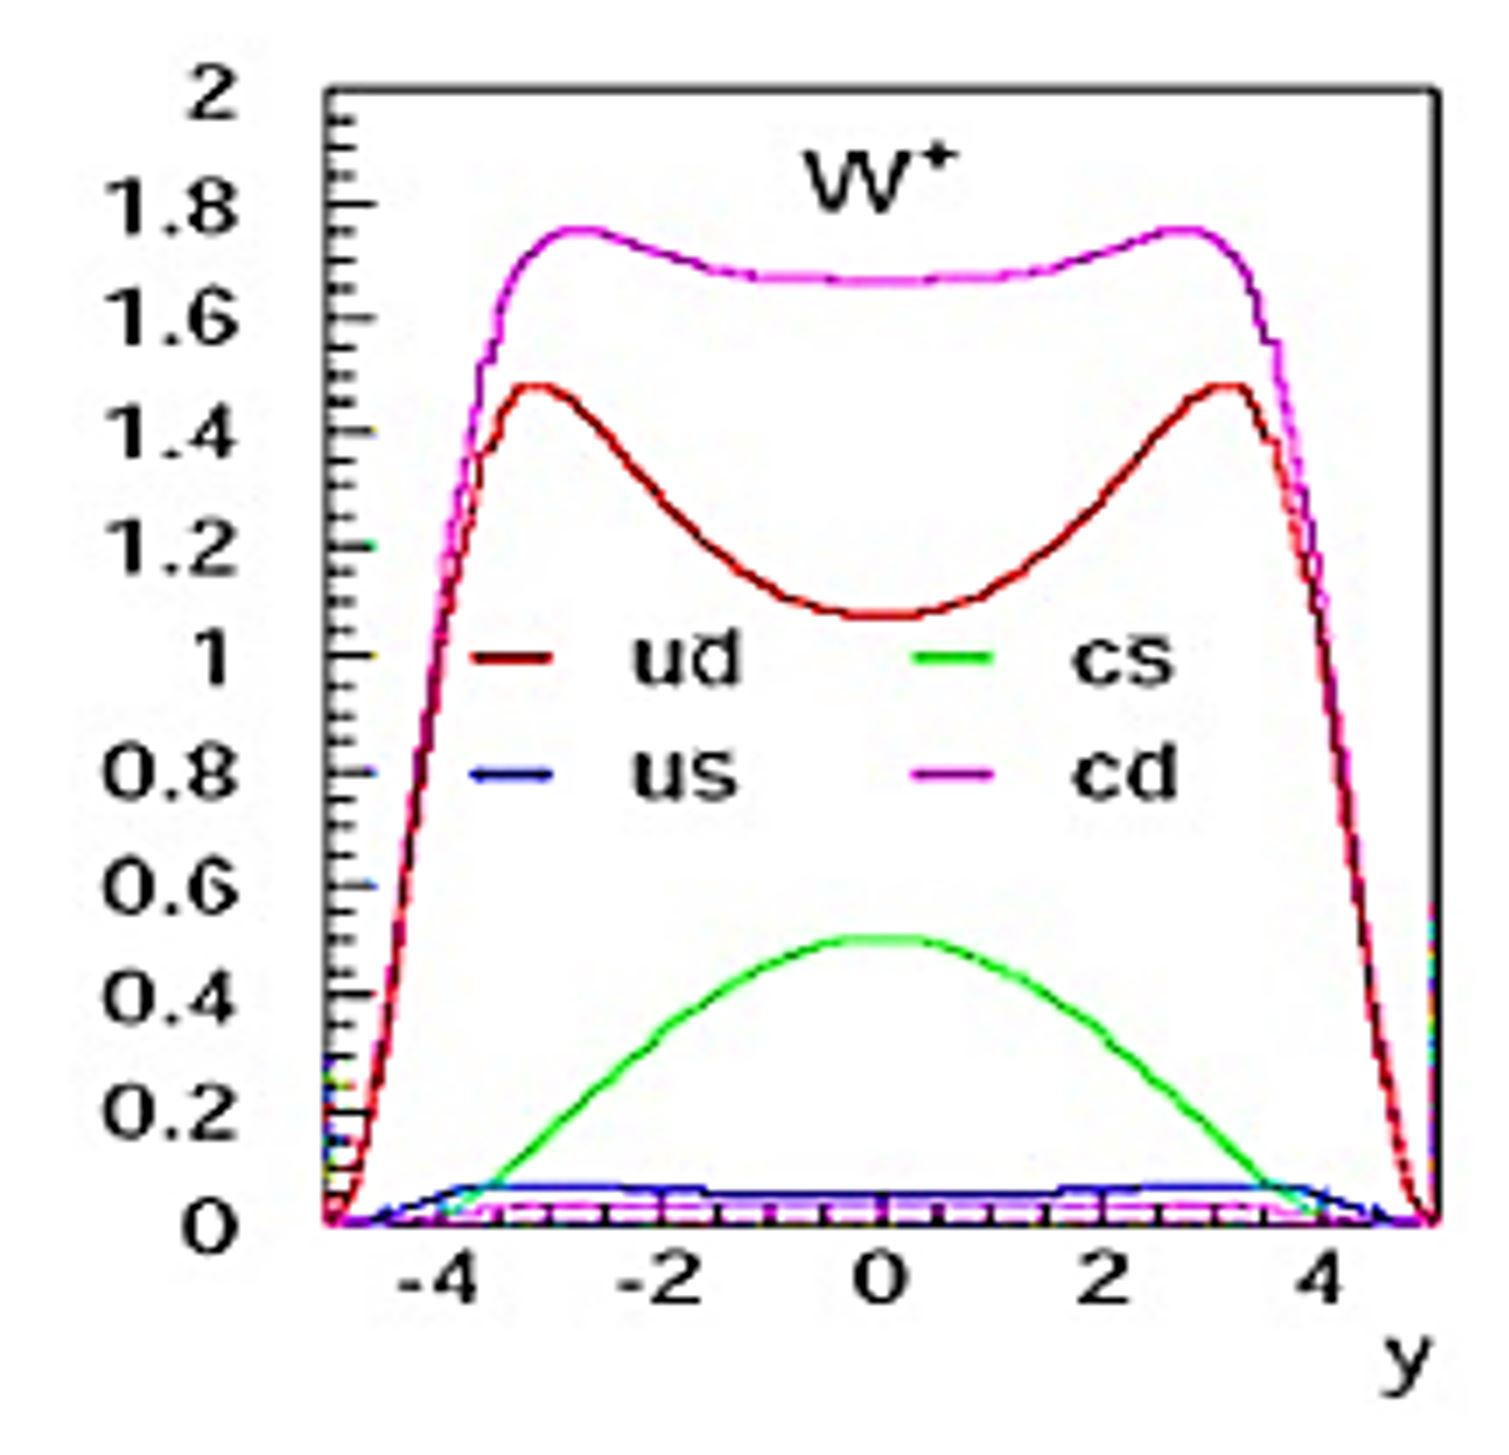
\includegraphics[width=0.31\textwidth]{plots/SM/rapidity_Wp.JPG}
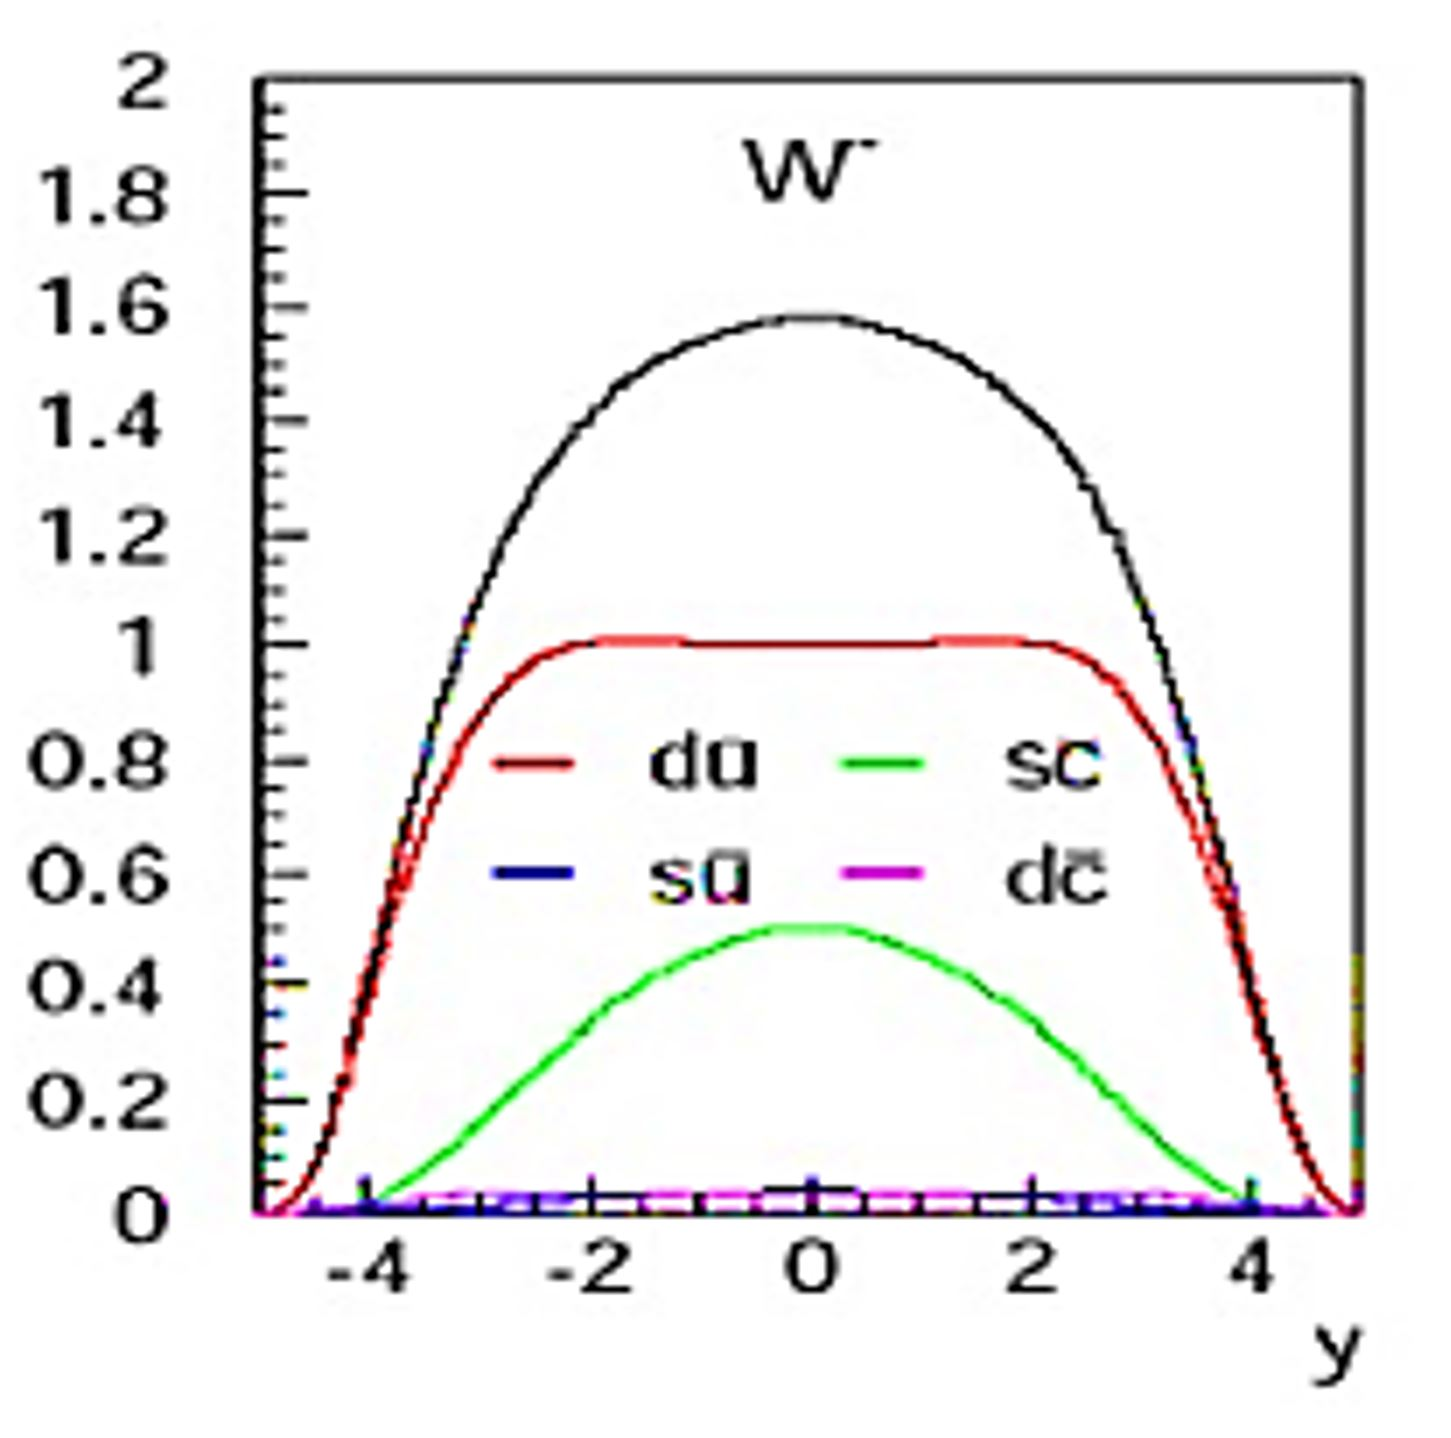
\includegraphics[width=0.30\textwidth]{plots/SM/rapidity_Wm.JPG}
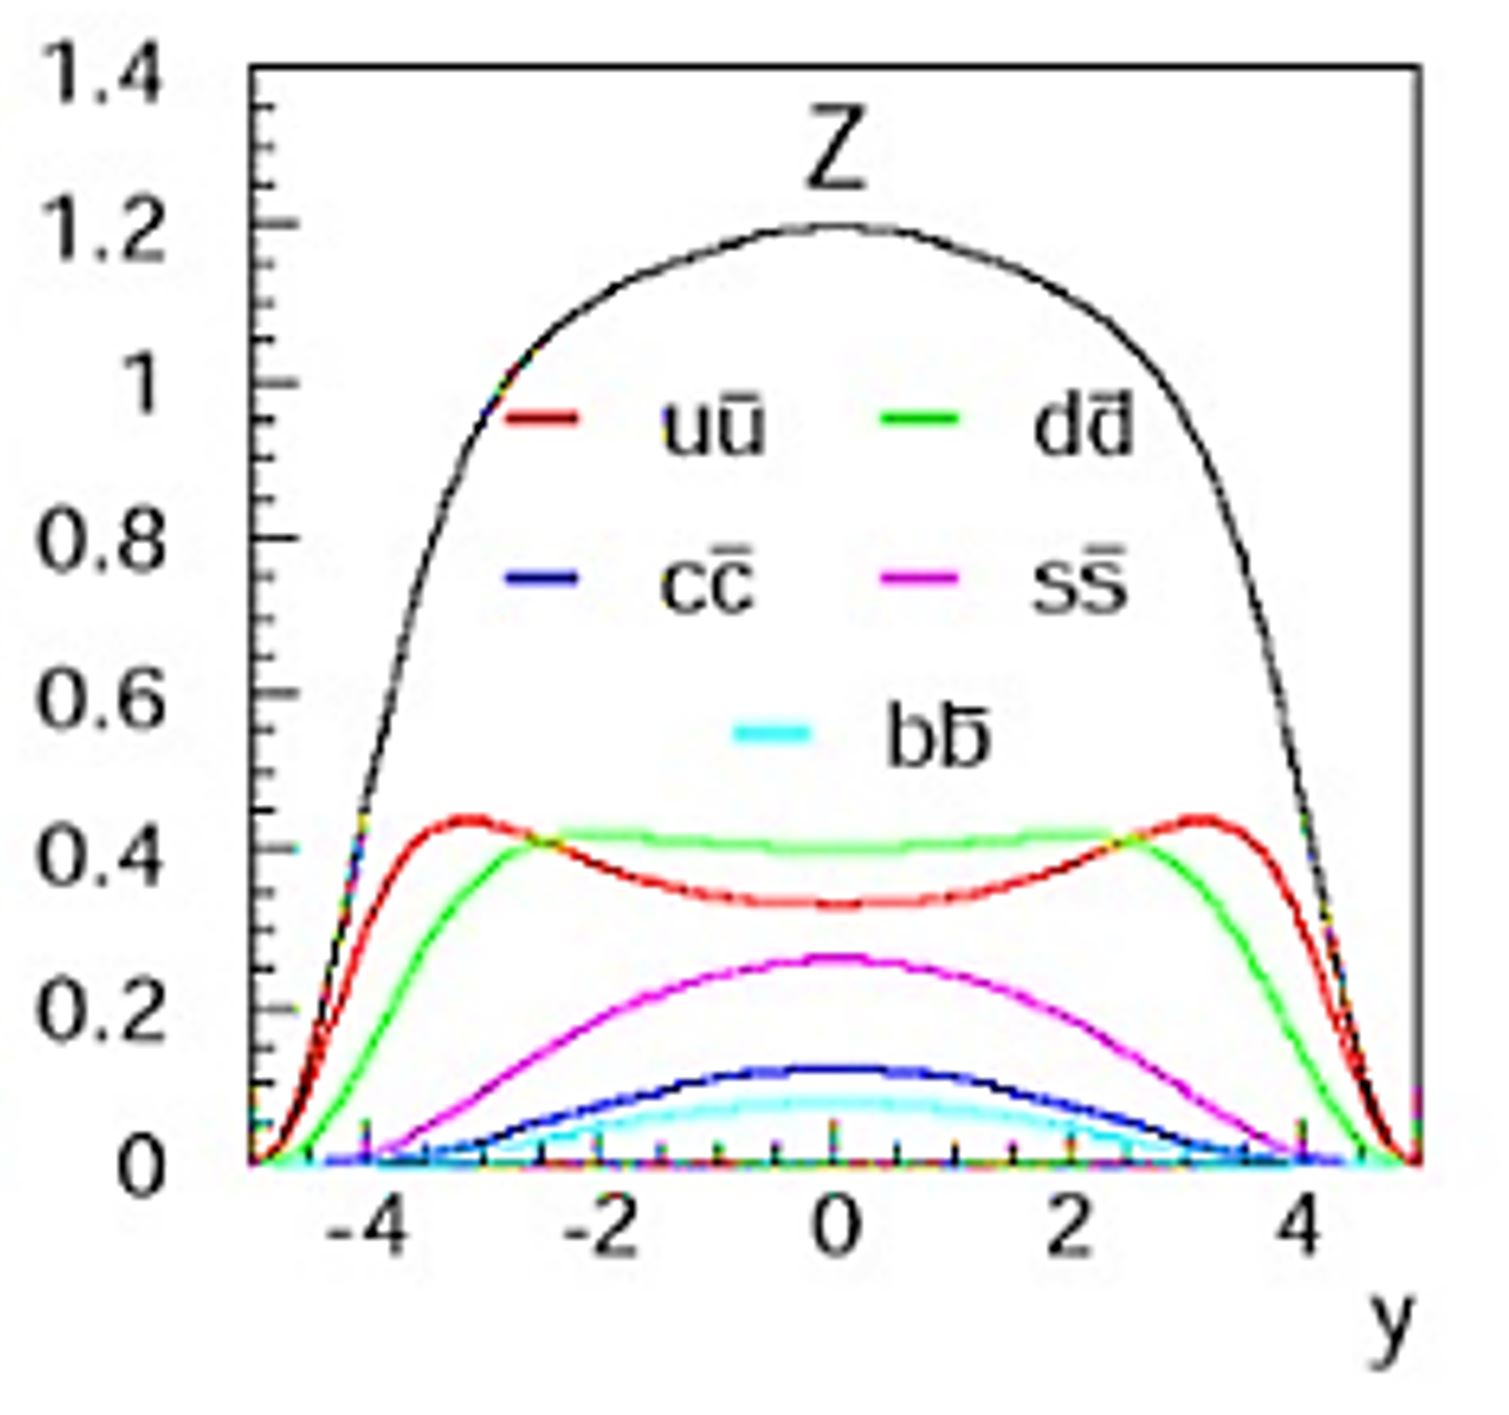
\includegraphics[width=0.32\textwidth]{plots/SM/rapidity_Z.JPG}
\caption{[Trying to make a new version from webplotdigitizer because these are ugly] Contribution of different quark flavors to the \Wp, \Wm, and \Z boson production over a range of boson rapidities. \Wp (\Wm) boson production is predominantly $u\bar{d}$ ($\bar{u}d$), while \Z boson production includes larger contributions from heavier flavors.}
\label{fig:wz_rapidity}
\end{figure}

%%%%%%%%%% ^^^^^ Section needs to be finished

%% Comment back in later if I feel like finishing

% \subsection{Simulating \pp collisions[need some work]}
% Practical descriptions of theoretical predictions are provided by Monte Carlo event generators. These generators rely on the approximations and factorization schemes that were described earlier in this section. Many collaborations dedicated to event generation tools exist, and are important in the era of LHC physics. The event generators come in generally two types: matrix element generators and parton shower generators. The matrix-element generators are distinguished by the order in $\alpha_s$ to which they provide calculations. 
% \begin{itemize}
%     \item \textbf{Pythia}: Pythia is a general-purpose event generator and can do both matrix-element calculation as well as initial and final state radiation and multiparton interactions. Pythia is often interfaced to other matrix-element calculators, where it provides the parton showering and hadronization steps, as done for the samples used in this analysis. \cite{Sjostrand:2014zea}
%     \item \textbf{aMC@NLO} MadGraph5\_aMC@NLO is a generator which provides matrix element calculations with up to two additional partons in the final state. This uses the NNPDF3.1 NLO PDF set.
%     \item \textbf{ResBos} 
%     \item \textbf{Powheg}
% \end{itemize}


% Predictions from event generators have uncertainties from several sources. Low-energy QCD processes which are dominiated by non-perturabtive effects are not well modeled and have large uncertainties. Parton showering is limited by its reliance on approximations. Proton PDFs have uncertainties. Additional uncertainty comes from higher-order terms in both QCD and QED, which are currently used at NNLO and LO. 

% PDF  uncertainties - general comment
% include multiple error sets reflecting the best fit with 1 sigma variations on the all of the params in the fit
% reflect uncertainties in data also
% inherent systematics dependent on way global fit is set up


% better predicionts of ewk mixing angle, w mass etc
